%%%%%%%%%%%%%%%%%%%%%%%%%%%%%%%%%%%%%%%%%%%%%%%%%%%%%%%%%%%%%%%%%%%%
%%%%%%%%%%%%%%%%%%%%%%%%%%%%%%%%%%%%%%%%%%%%%%%%%%%%%%%%%%%%%%%%%%%%
%%                                                                %%
%% Esimerkki opinnäytteen tekemisestä LaTeX:lla 20130926          %%
%% Alkuperäinen versio Luis Costa,  muutokset Perttu Puska        %%
%%                                                                %%
%% Tähän esimerkkiin kuuluu tiedostot                             %%
%%               opinnaytepohja.tex (versio 1.7)                  %%
%%               aaltothesis.sty (versio 1.7)                     %%
%%               kuva1.eps                                        %%
%%               kuva2.eps                                        %%
%%                                                                %%
%%                                                                %%
%% Kääntäminen                                                    %%
%% latex:                                                         %%
%%             $ latex opinnaytepohja                             %%
%%             $ latex opinnaytepohja                             %%
%%                                                                %%
%%   Tuloksena on tiedosto opinnayte.dvi, joka                    %%
%%   muutetaan ps-muotoon seuraavasti                             %%
%%                                                                %%
%%             $ dvips opinnaytepohja -o                          %%
%%                                                                %%
%% Selittävät kommentit on tässä esimerkissä varustettu           %%
%% %%-merkeillä ja muutokset, joita käyttäjä voi tehdä,           %%
%% on varustettu %-merkeillä                                      %%
%%                                                                %%
%%%%%%%%%%%%%%%%%%%%%%%%%%%%%%%%%%%%%%%%%%%%%%%%%%%%%%%%%%%%%%%%%%%%
%%%%%%%%%%%%%%%%%%%%%%%%%%%%%%%%%%%%%%%%%%%%%%%%%%%%%%%%%%%%%%%%%%%%

%% Käytä toinen näistä, jos kirjoitat suomeksi:
%% ensimmäinen, jos käytät pdflatexia (kuvat on oltava pdf-tiedostoina)
%% toinen, jos haluat tuottaa ps-tiedostoa (käytä eps-formaattia kuville).
%%
%% Use one of these you write in Finnish:
%% the 1st when using pdflatex (use pdf figures) or
%% the 2nd when producing a ps file (use eps figures).
\documentclass[finnish,12pt,a4paper,pdftex]{article}
%\documentclass[finnish,12pt,a4paper,dvips]{article}


%% Käytä näitä, jos kirjoitat englanniksi
%%
%% Uncomment one of these if you write in English
%\documentclass[english,12pt,a4paper,pdftex]{article}
%\documentclass[english,12pt,a4paper,dvips]{article}

%% Tämä paketti on pakollinen
%% Valitse korkeakoulusi näistä: arts, biz, chem, elec, eng, sci.
%% Valiste editorisi käyttämä merkkikoodaustapa: utf8, latin1
%%
%% This package is required
%% Choose your school from arts, biz, chem, elec, eng, sci.
%% Choose the character encoding scheme used by your editor: utf8, latin1
\usepackage[sci,utf8]{aaltothesis} % this is the default in aaltothesis.sty
%\usepackage[elec,latin1]{aaltothesis}

%% Jos käytät latex-komentoa käännettäessä (oletusarvo), 
%% kuvat kannattaa tehdä eps-muotoon. Älä käytä ps-muotoisia kuvia!
%% Käytä seuraavaa latex-komennon ja eps-kuvien kanssa 
%%
%% Jos taas käytät pdflatex-komentoa, joka kääntää tekstin suoraan
%% pdf-tiedostoksi, kuvasi on oltava jpg-formaatissa tai pdf-formaatissa.
%%
%% Use this if you run pdflatex and use jpg/pdf-format pictures.
%%
\usepackage{graphicx}

%% Jos et jostain syystä pidä, miten alla oleva hyperref-paketti käyttää
%% fontteja, värejä yms., käytä tämän paketin makroja muuttamaan
%% fonttimäärittelyt. Katso paketin dokumentaatiota. Paketti määrittelee
%% \url-makron, joten ota paketti käyttöön, jos et käytä hyperref-pakettia.
%%
%% Use the macros in this package to change how the hyperref package below 
%% typesets its hypertext -- hyperlink colour, font, etc. See the package
%% documentation. It also defines the \url macro, so use the package when 
%% not using the hyperref package.
%\usepackage{url}

%% Saat pdf-tiedoston viittaukset ja linkit kuntoon seuraavalla paketilla.
%% Paketti toimii erityisen hyvin pdflatexin kanssa. 
%%
%% Use this if you want to get links and nice output with pdflatex
%%
\usepackage[pdfpagemode=None,colorlinks=true,urlcolor=red,%
linkcolor=blue,citecolor=black,pdfstartview=FitH]{hyperref}

\usepackage[round]{natbib}
\bibliographystyle{agsm}

%% Matematiikan fontteja, symboleja ja muotoiluja lisää, näitä tarvitaan usein 
%%
%% Use this if you write hard core mathematics, these are usually needed
\usepackage{amsfonts,amssymb,amsbsy}  

%% Vaakasuunnan mitat, ÄLÄ KOSKE!
\setlength{\hoffset}{-1in}
\setlength{\oddsidemargin}{35mm}
\setlength{\evensidemargin}{25mm}
\setlength{\textwidth}{15cm}
%% Pystysuunnan mitat, ÄLÄ KOSKE!
\setlength{\voffset}{-1in}
\setlength{\headsep}{7mm}
\setlength{\headheight}{1em}
\setlength{\topmargin}{25mm-\headheight-\headsep}
\setlength{\textheight}{23cm}


%% Kaikki mikä paperille tulostuu, on tämän jälkeen
%%
%% Output starts here
\begin{document}

%% Korjaa vastaamaan korkeakouluasi, jos automaattisesti asetettu nimi on 
%% virheellinen 
%%
%% Change the school field to describe your school if the autimatically 
%% set name is wrong
% \university{aalto University}{aalto-Yliopisto}
% \school{School of Science}{Perustieteiden korkeakoulu}

%% Vain kandityölle: Korjaa seuraavat vastaamaan koulutusohjelmaasi
%%
%% Only for B.Sc. thesis: Choose your degree programme. 
%%\degreeprogram{Electronics and electrical engineering}%
%%{Elektroniikka ja sähkötekniikka}
%%

%% Vain DI/M.Sc.- ja lisensiaatintyölle: valitse laitos, 
%% professuuri ja sen professuurikoodi. 
%%
%% Only for M.Sc. and Licentiate thesis: Choose your department,
%% professorship and professorship code. 
%%\department{Department of Radio Science and Technology}%
%%{Radiotieteen ja -tekniikan laitos}
\professorship{ICT Business}{ICT liiketoiminta}
\code{???}
%%

%% Valitse yksi näistä kolmesta
%%
%% Choose one of these:
%\univdegree{BSc}
\univdegree{MSc}
%\univdegree{Lic}

%% Oma nimi
%%
%% Should be self explanatory...
\author{Jaakko Lehtinen}

%% Opinnäytteen otsikko tulee vain tähän. Älä tavuta otsikkoa ja
%% vältä liian pitkää otsikkotekstiä. Jos latex ryhmittelee otsikon
%% huonosti, voit joutua pakottamaan rivinvaihdon \\ kontrollimerkillä.
%% Muista että otsikkoja ei tavuteta! 
%% Jos otsikossa on ja-sana, se ei jää rivin viimeiseksi sanaksi 
%% vaan aloittaa uuden rivin.
%% 
%% Your thesis title. If the title is very long and the latex 
%% does unsatisfactory job of breaking the lines, you will have to
%% break the lines yourself with \\ control character. 
%% Do not hyphenate titles.
\thesistitle{Thesis template}{LISÄÄ NIMI}

\place{Espoo}
%% Kandidaatintyön päivämäärä on sen esityspäivämäärä! 
%% 
%% For B.Sc. thesis use the date when you present your thesis. 
\date{KORJAA: 24.9.2013}

%% Kandidaattiseminaarin vastuuopettaja tai diplomityön valvoja.
%% Huomaa tittelissä "\" -merkki pisteen jälkeen, 
%% ennen välilyöntiä ja seuraavaa merkkijonoa. 
%% Näin tehdään, koska kyseessä ei ole lauseen loppu, jonka jälkeen tulee 
%% hieman pidempi väli vaan halutaan tavallinen väli.
%%
%% B.Sc. or M.Sc. thesis supervisor 
%% Note the "\" after the comma. This forces the following space to be 
%% a normal interword space, not the space that starts a new sentence. 
\supervisor{Prof.\ Martti Mäntylä}{Prof.\ Martti Mäntylä}

%% Kandidaatintyön ohjaaja(t) tai diplomityön ohjaaja(t)
%% 
%% B.Sc. or M.Sc. thesis advisors(s). 
%%
%% Note that there has been a change in the official EN translation
%% of the Finnish title ``ohjaaja'' which in the previous version (1.5) 
%% of this document was called ``instructor''. The recommended
%% translation is now ``advisor''.  
%% However, the LaTeX internal variable remains \instructor
%% as there is little point to change the variable name. 
%%
%\instructor{Prof. Pirjo Professori}{Prof. Pirjo Professori}
%\instructor{D.Sc.\ (Tech.) Olli Ohjaaja}{TkT Olli Ohjaaja}
\instructor{M.Sc.\ (Tech.) Tapio Jakola}{DI Tapio Jakola}

%% Aaltologo: syntaksi:
%% \uselogo{aaltoRed|aaltoBlue|aaltoYellow|aaltoGray|aaltoGrayScale}{?|!|''}
%% Logon kieli on sama kuin dokumentin kieli
%%
%% Aalto logo: syntax:
% \uselogo{aaltoRed|aaltoBlue|aaltoYellow|aaltoGray|aaltoGrayScale}{?|!|''}
%% Logo language is set to be the same as the document language.
\uselogo{aaltoRed}{''}

%% Tehdään kansilehti
%%
%% Create the coverpage
\makecoverpage


%% Suomenkielinen tiivistelmä
%% 
%% Finnish abstract
%%
%% Tiivistelmän avainsanat
\keywords{Avainsanoiksi valitaan kirjoituksen sisältöä keskeisesti kuvaavia
käsitteitä}
%% Tiivistelmän tekstiosa
\begin{abstractpage}[finnish]
  Tiivistelmässä on lyhyt selvitys (noin 100 sanaa)
  kirjoituksen tärkeimmästä sisällöstä: mitä ja miten on tutkittu,
  sekä mitä tuloksia on saatu. 
  Tiivistelmässä on lyhyt selvitys (noin 100 sanaa)
  kirjoituksen tärkeimmästä sisällöstä: mitä ja miten on tutkittu,
  sekä mitä tuloksia on saatu. 

  Tiivistelmässä on lyhyt selvitys (noin 100 sanaa)
  kirjoituksen tärkeimmästä sisällöstä: mitä ja miten on tutkittu,
  sekä mitä tuloksia on saatu. 
  Tiivistelmässä on lyhyt selvitys (noin 100 sanaa)
  kirjoituksen tärkeimmästä sisällöstä: mitä ja miten on tutkittu,
  sekä mitä tuloksia on saatu. 
  Tiivistelmässä on lyhyt selvitys (noin 100 sanaa)
  kirjoituksen tärkeimmästä sisällöstä: mitä ja miten on tutkittu,
  sekä mitä tuloksia on saatu. 
\end{abstractpage}

%% Pakotetaan uusi sivu varmuuden vuoksi, jotta 
%% mahdollinen suomenkielinen ja englanninkielinen tiivistelmä
%% eivät tule vahingossakaan samalle sivulle
%%
%% Force new page so that English abstract starts from a new page
\newpage
%
%% English abstract, uncomment if you need one. 
%% 
%% Abstract keywords
\keywords{}
%% Abstract text
\begin{abstractpage}[english]
 Your abstract in English. Try to keep the abstract short, approximately 
 100 words should be enough. Abstract explains your research topic, 
 the methods you have used, and the results you obtained.  
\end{abstractpage}
%% Note that 
%% if you are writting your master's thesis in English place the English
%% abstract first followed by the possible Finnish abstract

%% Esipuhe 
%%
%% Preface
\mysection{Esipuhe}
%\mysection{Preface}
Lisää tähän esipuhe.\\

\vspace{5cm}
Otaniemi, 24.9.2013

\vspace{5mm}
{\hfill T T.\ A.\ Teekkari \hspace{1cm}}

%% Pakotetaan varmuuden vuoksi esipuheen jälkeinen osa
%% alkamaan uudelta sivulta
%%
%% Force new page after preface
\newpage


%% Sisällysluettelo
%% 
%% Table of contents. 
\thesistableofcontents


%% Symbolit ja lyhenteet
%%
%% Symbols and abbreviations
\mysection{Symbolit ja lyhenteet (Esimerkki)}
%\mysection{Symbols and abbreviations}
\subsection*{Symbolit}
%\subsection*{Symbols}

\begin{tabular}{ll}
%$|a_{ij}|^2$, $|a_i|^2$ & probability of two electrons having momenta
%    $\boldsymbol p_i$ and $\boldsymbol p_j$ ($\boldsymbol p_i$ for $|a_i|^2$) \\
%                 & at any given instant \\
$\mathbf{B}$  & magneettivuon tiheys  \\
$c$              & valon nopeus tyhjössä $\approx 3\times10^8$ [m/s]\\
%$p$              & magnitude of momentum \\
%$\boldsymbol p$, $\boldsymbol p_i$, $\boldsymbol p_i^{'}$  & momentum vector \\
%$p$              & magnitude of momentum \\
%$\boldsymbol p$, $\boldsymbol p_i$, $\boldsymbol p_i^{'}$  & momentum vector \\
%$\boldsymbol P$  &  \\
%$p_{\mathrm{F}}$ & Fermi momentum \\
$\omega_{\mathrm{D}}$    & Debye-taajuus \\
$\omega_{\mathrm{latt}}$ & hilan keskimääräinen fononitaajuus \\
$\uparrow$       & elektronin spinin suunta ylöspäin\\
$\downarrow$     & elektronin spinin suunta alaspäin
\end{tabular}

\subsection*{Operaattorit}
%\subsection*{Opetators}

\begin{tabular}{ll}
$\nabla \times \mathbf{A}$              & vektorin $\mathbf{A}$ roottori\\
$\displaystyle\frac{\mbox{d}}{\mbox{d} t}$ & derivaatta muuttujan $t$ suhteen\\
[3mm]
$\displaystyle\frac{\partial}{\partial t}$  & osittaisderivaatta muuttujan $t$ suhteen \\[3mm]
$\sum_i $                       & Summa indeksin $i$ yli\\
$\mathbf{A} \cdot \mathbf{B}$    & vektorien $\mathbf{A}$ ja $\mathbf{B}$ pistetulo
\end{tabular}

\subsection*{Lyhenteet}
%\subsection*{Abbreviations}

\begin{tabular}{ll}
AC         & vaihtovirta \\
APLAC      & an object-oriented analog circuit simulator and design tool \\
           & (originally Analysis Program for Linear Active Circuits) \\
BCS        & Bardeen-Cooper-Schrieffer \\ %% tavuviiva - nimien välissä 
DC         & tasavirta \\
TEM        & transverse eletromagnetic
\end{tabular}


%% Sivulaskurin viilausta opinnäytteen vaatimusten mukaan:
%% Aloitetaan sivunumerointi arabialaisilla numeroilla (ja jätetään
%% leipätekstin ensimmäinen sivu tyhjäksi, 
%% ks. alla \thispagestyle{empty}).
%% Pakotetaan lisäksi ensimmäinen varsinainen tekstisivu alkamaan 
%% uudelta sivulta clearpage-komennolla. 
%% clearpage on melkein samanlainen kuin newpage, mutta 
%% flushaa myös LaTeX:n floatit 
%% 
%% Corrects the page numbering, there is no need to change these
\cleardoublepage
\storeinipagenumber
\pagenumbering{arabic}
\setcounter{page}{1}


%% Leipäteksti alkaa
%%
%% Text body begins. Note that since the text body
%% is mostly in Finnish the majority of comments are
%% also in Finnish after this point. There is no point in explaining
%% Finnish-language specific thesis conventions in English.
\section{Johdanto}
%\section{Introduction}

%% Ensimmäinen sivu tyhjäksi
%% 
%% Leave first page empty
\thispagestyle{empty}

Yrityksen tulee etsiä tapoja säästää resursseja ja mahdollistaa itsepalvelu sen asiakkaille kellonajasta riippumatta, ja nämä tavoitteet ovat parhaiten saavutettavissa IT-palvelujen ja prosessessien automatisoinnilla \citep{lamoureux}. Yritykset aloittivat mekaanisen automatisoinnin jo 1950-luvulla, ja jokainen teknologinen kehitysaskel sen jälkeen on mahdollistanut yhä monimutkaisempien toimintojen automatisoinnin yrityksen toiminnassa.

Automaatio käsitteenä sai merkityksensä autoteollisuuden tuotantolinjoilta, ja tietotekniikan yleistymisen jälkeen 1970-ja 1980-luvulla yritykset oppivat hyödyntämään automaatiota myös sisäisissä, laskentaa vaativissa prosesseissa, kuten taloushallinnossa. Internetin yleistymisen myötä 1990-2000-luvuilla teknologian kehitys on mahdollistanut liiketoimintaprosessien automatisoinnin. Koko tilaus- ja toimitusketju ja useat tuotteet ja palvelut muuttuivat digitaalisiksi. Automaatiossa ei ole siis pelkästään kysymys ihmistyön antamisesta tietokoneelle, vaan myös sen tekemisestä mikä ei aikaisemmin ollut mahdollista \citep{groover}.


Mitä automaatio tarkoittaa tässä ajassa

Palveluilta ja tuotteilta odotetaan että ne saadaan käyttöön nopeasti, ja että niiden käytön aloittaminen on helppoa itsepalveluna. Amazon verkkokauppajätti onnistui tässä yhtenä ensimmäisistä ja on siten näyttänyt tietä perinteisille kaupan alan toimijoille, että on kannattavaa soveltaa digitaalisia teknologioita kehittääkseen tuotteita ja palveluita asiakkaille, sisäisiä prosesseja ja asiakaskokemusta. Yhteyksien nopeutumisen ja teknologisen kehityksen myötä sama ilmiö on levinnyt muillekin alueille. Fyysiset tuotteet ja palvelut siirtyvät digitaaliseen muotoon. Musiikkia tai elokuvia ei tarvitse ladata tai ostaa enää, vaan ne ovat käytettävissä pilvipalveluiden kautta välittömästi jokaiselle laitteelle. Tämä on johtanut siihen, että kaiken pitää olla helposti saatavilla myös yritysmaailmassa joukolle erilaisia päätelaitteita.

Teknologinen kehitys on johtanut siihen, että saatavilla olevia teknologioita on koko ajan eksponentiaalisesti enemmän, ja teknologiat ovat yhä kompleksimpia. Taustalla olevat koko ajan kompleksisemmat teknologiat kuitenkin näyttäytyvät simppelinä käyttäjälle. Esimerkiksi palvelut ja tuotteet voidaan nähdä näytelmänä teatterissa. Näytelmän monimutkaiset käänteet osataan esittää ja tarjoilla yhä helpommin yleisölle nautittavaksi uuden teknologian ansiosta, mutta yleisö ei näe mitä näyttämön lavan takana tapahtuu. 
Monimutkaisuuden tiivistäminen helposti esitettävään muotoon vaatii yhä kasvavan osien määrän orkestrointia tehokkaasti. Osaset tai resurssit lavan takana aiheuttavat kustannuksia, joiden perusteella näytelmän liput hinnoitellaan. Asiakkaat haluavat elämyksiä, joita on tarjolla useissa teattereissa. Siksi kohtuullinen ja kilpailukykyinen hinta on tärkeä asia. Säilyäkseen mukana kilpailussa on siis tärkeä pohtia mahdollisuuksia pienentää kustannuksia, eli saavuttaa päämäärä pienemmillä resursseilla. Aikaisemmassa esimerkissä Amazon onnistui disruptoimaan markkinoita kehittämällä digitaaliset liiketoiminnan prosessit, eli se antoi tietokoneelle suoritettavaksi tehtäviä, jotka sen kilpailijat suorittivat ihmisvoimin. 

Digitaalisuus on siis fyysisen muuttumista

Siksi onkin luonnollista automatisoida prosessit lavan takana, jolloin orkestrointi on helpompaa ja vaatii vähemmän resursseja. Automatisointi suoritetaan teknologian avulla, jolloin tietokone suorittaa tehtävät aina samalla tavalla ja samalla laadulla. 
organisointia ja tehokkuutta lavan takana. 
Disruptor disrupted,

Trendit:\\
Automaatio, RPA, Lean, Nopeasti pilvestä yms. \\

Nykytilanne:\\
Näkökulma, josta työn ongelmaa lähestytään, on haasteet saman tuotealueen järjestelmien tilaus-, toimitus- ja laskutusprosesseissa. Asiakastoimitukset vaativat usein oman projektinsa suuren työmäärän hallinnoimiseksi, joka on suurelta osin manuaalista työtä. Toimitusajat ovat usein viikoista kuukausiin, ja samalla asiakaslaskutuksen aloittaminen viivästyy. Suuresta työmäärästä, pitkistä toimitusajoista ja laskutuksen viivästymisestä johtuen kustannukset ovat korkeat. Tällöin kärsii myös kyky vastata asiakkaiden tarpeisiin ja kasvattaa asiakastyytyväisyyttä.



Telialla kyseinen asiakaspalvelujärjestelmä mielletään kompleksisena. Kompleksi tarkoittaa tässä yhteydessä sitä, että toimiakseen se vaatii runsaasti integrointeja ja konfigurointia asiakaskohtaisesti. Tämä työ on usein manuaalista, ja tietotaito sen tekemisestä keskittyy rajatulle määrälle henkilöitä.
Organisaatio toivoo automaation olevan ratkaisu monien ongelmien ratkaisuun, ja pyrkimyksiä automaation lisäämiseen on nähtävissä. Tavoitteena on lisätä merkittävästi itsepalvelua, aloittaa laskutus mahdollisimman nopeasti tilauksesta, toimia kustannustehokkaasti ja lisätä asiakastyytyväisyyttä. Automaatiota lisäävien ratkaisujen tulisi olla monistettavissa muihinkin vastaaviin prosesseihin.\\

Transformaatiosta jotain? front-end(salesforce, ei enää exceleitä)/back-end(integraatio, robotiikka, legacy)\\


Teoreettinen viitekehys:\\
BPA, RPA, Lean, ...
Prosessin automatisointia tarkastellaan....
Tämä onnistuu hyödyntämällä teoriaa liiketoimintaprosessien automatisoinnista, ohjelmistorobotiikasta ja Lean-ajattelusta nykyisessä liiketoimintakontekstissa.\\

Tutkimuskysymys ja alakysymykset:
\begin{itemize}
\item[--]Miten asiakaspalvelujärjestelmän tilaus-, toimitus- ja laskutusprosessi tulisi automatisoida nykyisessä liiketoimintakontekstissa?
\end{itemize}

Pääkysymykseen vastataan alakysymysten avulla, alakysymyksiksi olen valinnut:
\begin{itemize}
\item[--]Kysymys X
\item[--]Kysymys Y
\end{itemize}

Tutkimuksen rajaus:\\
Työssä keskitytään pohtimaan kyseisen prosessin automatisointia, joten johtopäätökset eivät päde täysin muiden prosessien kohdalla. Tästä huolimatta työssä on pohdintaa prosessin eri osien automatisoinnin hyödyntämisessä myös muualla organisaatiossa.

%% Opinnäytteessä jokainen osa alkaa uudelta sivulta, joten \clearpage
%%
%% In a thesis, every section starts a new page, hence \clearpage
\clearpage

\section{Taustatieto}


% \section{Background}
\subsection{Asiakasprosessi ja sen automatisoinnin arvo}
\subsection{Asiakaspalvelujärjestelmät}
\subsection{Digitaalinen visio Telialla}




\clearpage

\section{Tutkimusaineisto ja -menetelmät}
%\section{Materials and methods}

Tässä osassa kuvataan käytetty tutkimusaineisto ja
tutkimuksen metodologiset valinnat, sekä
kerrotaan tutkimuksen toteutustapa ja käytetyt menetelmät. 

\clearpage

\section{Tulokset}
%\section{Results}

Tässä osassa esitetään tulokset ja vastataan tutkielman alussa
esitettyihin tutkimuskysymyksiin. Tieteellisen kirjoitelman
arvo mitataan tässä osassa esitettyjen tulosten perusteella. 

%% Huomaa seuraavassa kappaleessa lainausmerkkien ulkopuolella piste, 
%% koska piste ei lopeta lainattua tekstinpätkää.
%% Jos lainattu tekstinpätkä loppuu välimerkkiin, tulee välimerkki
%% lainausmerkkien sisälle: 
%% "Et tu, Brute?" sanoi Caesar kuollessaan.
Tutkimustuloksien merkitystä on aina syytä arvioida ja tarkastella
kriittisesti.  Joskus tarkastelu voi olla tässä osassa, mutta se
voidaan myös jättää viimeiseen osaan, jolloin viimeisen osan nimeksi
tulee >>Tarkastelu>>. Tutkimustulosten merkitystä voi arvioida myös
>>Johtopäätökset>>-otsikon alla viimeisessä osassa. 

Tässä osassa on syytä myös arvioida tutkimustulosten luotettavuutta.
Jos tutkimustulosten merkitystä arvioidaan >>Tarkastelu>>-osassa,
voi luotettavuuden arviointi olla myös siellä. 

\clearpage

\section{Yhteenveto}
%\section{Summary} 

Opinnäytteen tekijä vastaa siitä, että opinnäyte on tässä dokumentissa
ja opinnäytteen tekemistä käsittelevillä luennoilla sekä
harjoituksissa annettujen ohjeiden mukainen muotoseikoiltaan,
rakenteeltaan ja ulkoasultaan.



\clearpage
%% Lähdeluettelo
%%
%% \phantomsection varmistaa, että hyperref-paketti latoo hypertekstilinkit
%% oikein.
%%
%% The \phantomsection command is nessesary for hyperref to jump to the 
%% correct page, in other words it puts a hyper marker on the page.

\phantomsection
%\addcontentsline{toc}{section}{Viitteet}
%\addcontentsline{toc}{section}{References}
%%\begin{thebibliography}{99}
\bibliography{lahteet}

%% Alla pilkun jälkeen on pakotettu oikea väli \<välilyönti>-merkeillä.

%%\end{thebibliography}

%% Liitteet 
\appendix 
\clearpage
%% Lisää tekstin "Liitteet" sisällysluetteloon
%%
%% Adds the word "Appendices" to the table of contents
\addtocontents{toc}{\protect\contentsline{section}{Liiteet}{}{appendix}}
%\addtocontents{toc}{\protect\contentsline{section}{Appendices}{}{appendix}}

\section{Esimerkki liitteestä\label{LiiteA}}
%% Liitteiden kaavat, taulukot ja kuvat numeroidaan omana kokonaisuutenaan
%%
%% Equations, tables and figures have their own numbering in Appendices
\renewcommand{\theequation}{A\arabic{equation}}
\setcounter{equation}{0}  
\renewcommand{\thefigure}{A\arabic{figure}}
\setcounter{figure}{0}
\renewcommand{\thetable}{A\arabic{table}}
\setcounter{table}{0}

Liitteet eivät ole opinnäytteen kannalta välttämättömiä ja 
opinnäytteen tekijän on 
kirjoittamaan ryhtyessään hyvä ajatella pärjäävänsä ilman liitteitä.
Kokemattomat kirjoittajat, jotka ovat huolissaan
tekstiosan pituudesta, paisuttavat turhan 
helposti liitteitä pitääkseen tekstiosan pituuden annetuissa rajoissa.
Tällä tavalla ei synny hyvää opinnäytettä.   

Liite on itsenäinen kokonaisuus, vaikka se täydentääkin tekstiosaa.
Liite ei siten ole pelkkä listaus, kuva tai taulukko, vaan 
liitteessä selitetään aina sisällön laatu ja tarkoitus. 

Liitteeseen voi laittaa esimerkiksi listauksia. Alla on 
listausesimerkki tämän liitteen luomisesta. 

%% Verbatim-ympäristö ei muotoile tai tavuta tekstiä. Fontti on monospace.
%% Verbatim-ympäristön sisällä annettuja komentoja ei LaTeX käsittele. 
%% Vasta \end{verbatim}-komennon jälkeen jatketaan käsittelyä.
\begin{verbatim}
	\clearpage
	\appendix
	\addcontentsline{toc}{section}{Liite A}
	\section*{Liite A}
	...
	\thispagestyle{empty}
	...
	tekstiä
	...
	\clearpage
\end{verbatim}

Kaavojen numerointi muodostaa liitteissä oman kokonaisuutensa:
\begin{eqnarray}
d \wedge A  &=& F, \label{liitekaava1}\\
d \wedge F  &=& 0. \label{liitekaava2}
\end{eqnarray}


\clearpage
\section{Toinen esimerkki liitteestä\label{LiiteB}}

%% Liitteiden kaavat, taulukot ja kuvat numeroidaan omana kokonaisuutenaan
%%
%% Equations, tables and figures have their own numbering in Appendices
\renewcommand{\theequation}{B\arabic{equation}}
\setcounter{equation}{0}  
\renewcommand{\thefigure}{B\arabic{figure}}
\setcounter{figure}{0}
\renewcommand{\thetable}{B\arabic{table}}
\setcounter{table}{0}

Liitteissä voi myös olla kuvia, jotka
eivät sovi leipätekstin joukkoon:
%% Ympäristön figure parametrit htb pakottavat
%% kuvan tähän, eikä LaTeX yritä siirrellä niitä
%% hyväksi katsomaansa paikkaan. 
%% Ympäristöä center voi käyttää \centering-
%% komennon sijaan
%%
%% Example of a figure, note the use of htb parameters which force
%% the figure to be inserted here
\begin{figure}[htb]
\begin{center}
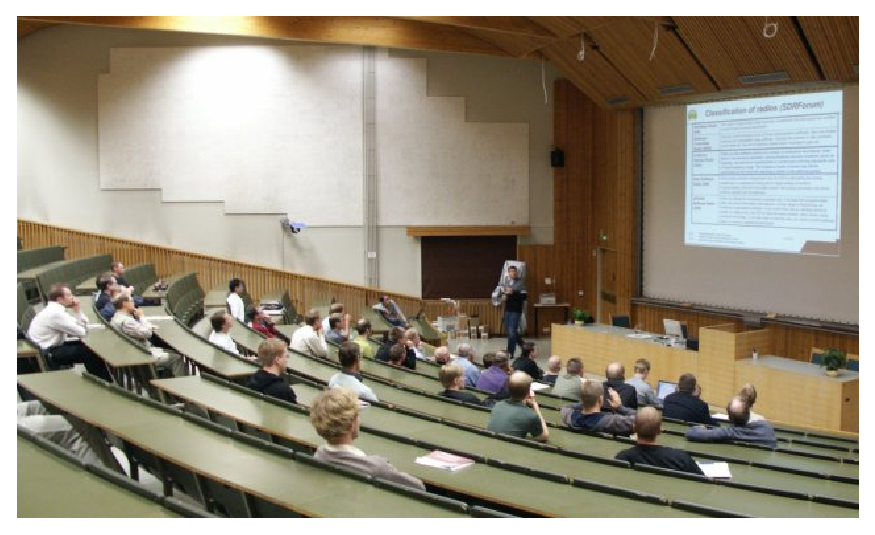
\includegraphics[height=8cm]{kuva2}
\end{center}
\caption{Kuvateksti, jossa on liitteen numerointi \label{liitekuva}}
\end{figure}
%%
Liitteiden taulukoiden numerointi on kuvien ja kaavojen kaltainen:
\begin{table}[htb]
\caption{Taulukon kuvateksti. \label{liitetaulukko}}
\begin{center}
\fbox{
\begin{tabular}{lp{0.5\linewidth}}
9.00--9.55  & Käytettävyystestauksen tiedotustilaisuus (osanottajat
ovat saaneet sähköpostitse valmistautumistehtävät, joten tiedotustilaisuus
voidaan pitää lyhyenä).\\
9.55--10.00 & Testausalueelle siirtyminen
\end{tabular}}
\end{center}
\end{table}
Kaavojen numerointi muodostaa liitteissä oman kokonaisuutensa:
\begin{eqnarray}
T_{ik} &=& -p g_{ik} + w u_i u_k + \tau_{ik},  \label{liitekaava3} \\
n_i    &=& n u_i + v_i.                        \label{liitekaava4}
\end{eqnarray}

\end{document}
